\chapter{Methods for Acoustic Characteristics Retrieval from Complex Virtual Environments} % If you're changing this, update Section 1.6
\label{ch:Materials}
The following Chapter introduces two systems to retrieve acoustic characteristics from space surrounding users in \acrshort{ar}, providing fundamental building blocks for subsequent acoustic rendering techniques to simulate sound transmissions between an entity in \acrshort{ar} space and the user. The acoustic characteristics extracted from the physical and virtual scene experienced by the user allow context-aware rendering, enabling the acoustic renderers discussed in Chapter~\ref{ch:acousticrendering} to approximate sound waves with geometrical primitives and compute propagation paths from sources to a listener, i.e., the user. Propagation paths, calculated by intersecting rays (or other primitives) with the environment, can respond to the physical properties of surfaces or scene entities, attributing characteristics to portions of the scene geometry. This allows propagation paths to model how acoustic energy propagating from an emitter in \acrshort{ar} space is affected by diverse surfaces in space, enabling context-aware auditory interactions.\par
The following Chapter is structured around two main sections presenting novel workflows for acoustic information retrieval:
\begin{enumerate}
    \item a \textbf{camera-based} system to understand complex scenes and project acoustic information based on visual renders,
    \item and a \textbf{texture-based} extension that improves the above by abstracting away from camera render and analyses texture data from scene geometry.
\end{enumerate}
The two methods predict acoustic characteristics of space from their visual representations to inform sound rendering and produce believable acoustic stimuli in interactive applications. The methods are tested on various complex scenes, ranging from authored virtual scenes to reconstructions of physical space with LiDAR scanners, emulating input environments that are typically available to \acrshort{ar} \acrshortpl{hmd}. The methods presented demonstrate applications of scene understanding techniques to virtual environments and digital reconstructions of real space to determine acoustic properties of scene geometry for automating realistic sound rendering, and they are evaluated on state-of-the-art acoustic rendering systems, measuring objective and subjective metrics relating to simulated soundfields.\par

\section{Introduction}
% Camera-based approach
Modern sound rendering, as discussed across Chapters~\ref{ch:litReview} and~\ref{ch:Background}, often requires the positions of sound sources and listeners, as well as the scene geometry with acoustic characteristics expressing the behaviour of each material. The accuracy of acoustic simulations depends on material information assigned to the scene geometry. The scene geometry, tagged with frequency-dependent absorption and scattering information, determines how sound behaves in space and affects the resulting wavefield. Attributing material characteristics to scene geometry segments and entities is commonly performed manually and often at a high cost and resources due to the human-in-the-loop.\par
In game development, for instance, tagging materials with appropriate acoustic data often requires the work of experts, raising costs and resource needs for large scenes. This Chapter illustrates progress towards creating an automatic process for the generation of material tagging data that can provide input to sound rendering pipelines. Specifically, here are proposed proof-of-concept systems for vision-based material information retrieval, allowing for tagging an object's acoustic properties based on its visual features. These systems can tag meshes in \acrshortpl{ve} representing boundaries in sound propagation paths with a noticeable perceptual impact, facilitating acoustic renderers on complex scenes. The goal is to remove the human-in-the-loop to allow virtual reconstructions of real space to provide input to acoustic rendering systems automatically.\par
At the core of these methods lies the problem of scene segmentation. In computer games, often, a set of meshes composes a scene, where each mesh represents an object in the scene. Acoustic materials are often assigned to all triangles composing a given mesh, allowing audio engineers to group scene geometry when assigning acoustic data. Hence, the resulting acoustic model's accuracy depends on the separation of the geometry, where ideal conditions would have each triangle mapped to its specific acoustic data. A naive approach would have the entire geometry mapping to a single acoustic material. Besides, the representation of materials in real and virtual environments adds further dimensions to the material tagging problem due to complex links between the visual representation of materials of an object and its perceptual effects on the soundscape of the environments in which it exists.\par
This Chapter addresses acoustic material tagging by providing the following contributions:
\begin{itemize}
    \item a novel methodology for acoustic material tagging using a camera-based system and computer vision techniques to infer from the scene;
    \item an alternative system that abstracts from the use of cameras and operates on reconstructed virtual geometry;
    \item objective and subjective methodologies to evaluate the efficacy of the systems comparing against objective and subjective metrics;
    \item a proof-of-concept demonstration stemming from the development of the two systems
\end{itemize}


\section{Camera-based Acoustic Material Tagging}\label{sec:camera-tagging}
\subsection{System Overview}
The camera-based acoustic material tagging pipeline is the first approach to attribute physical properties to portions of scene geometry representing a virtual environment. At a high-level overview, the pipeline adopts a \acrfull{cnn} to understand the scene features of the environment, expressed as pixel-wise semantic information predicted from camera renders obtained by a perspective camera within the virtual environment. The network generates a prediction map where pixel-wise semantic information maps to acoustic absorption information, e.g., a pixel belonging to a wooden table in the virtual scene may be attributed with ``wood'' semantics, which maps to absorption data related to the semantic material. By using camera transformation matrices, semantic information is projected onto the scene from camera space. The system has two phases: \emph{training} and \emph{inference}.
\begin{figure}[htbp]
    \centering
    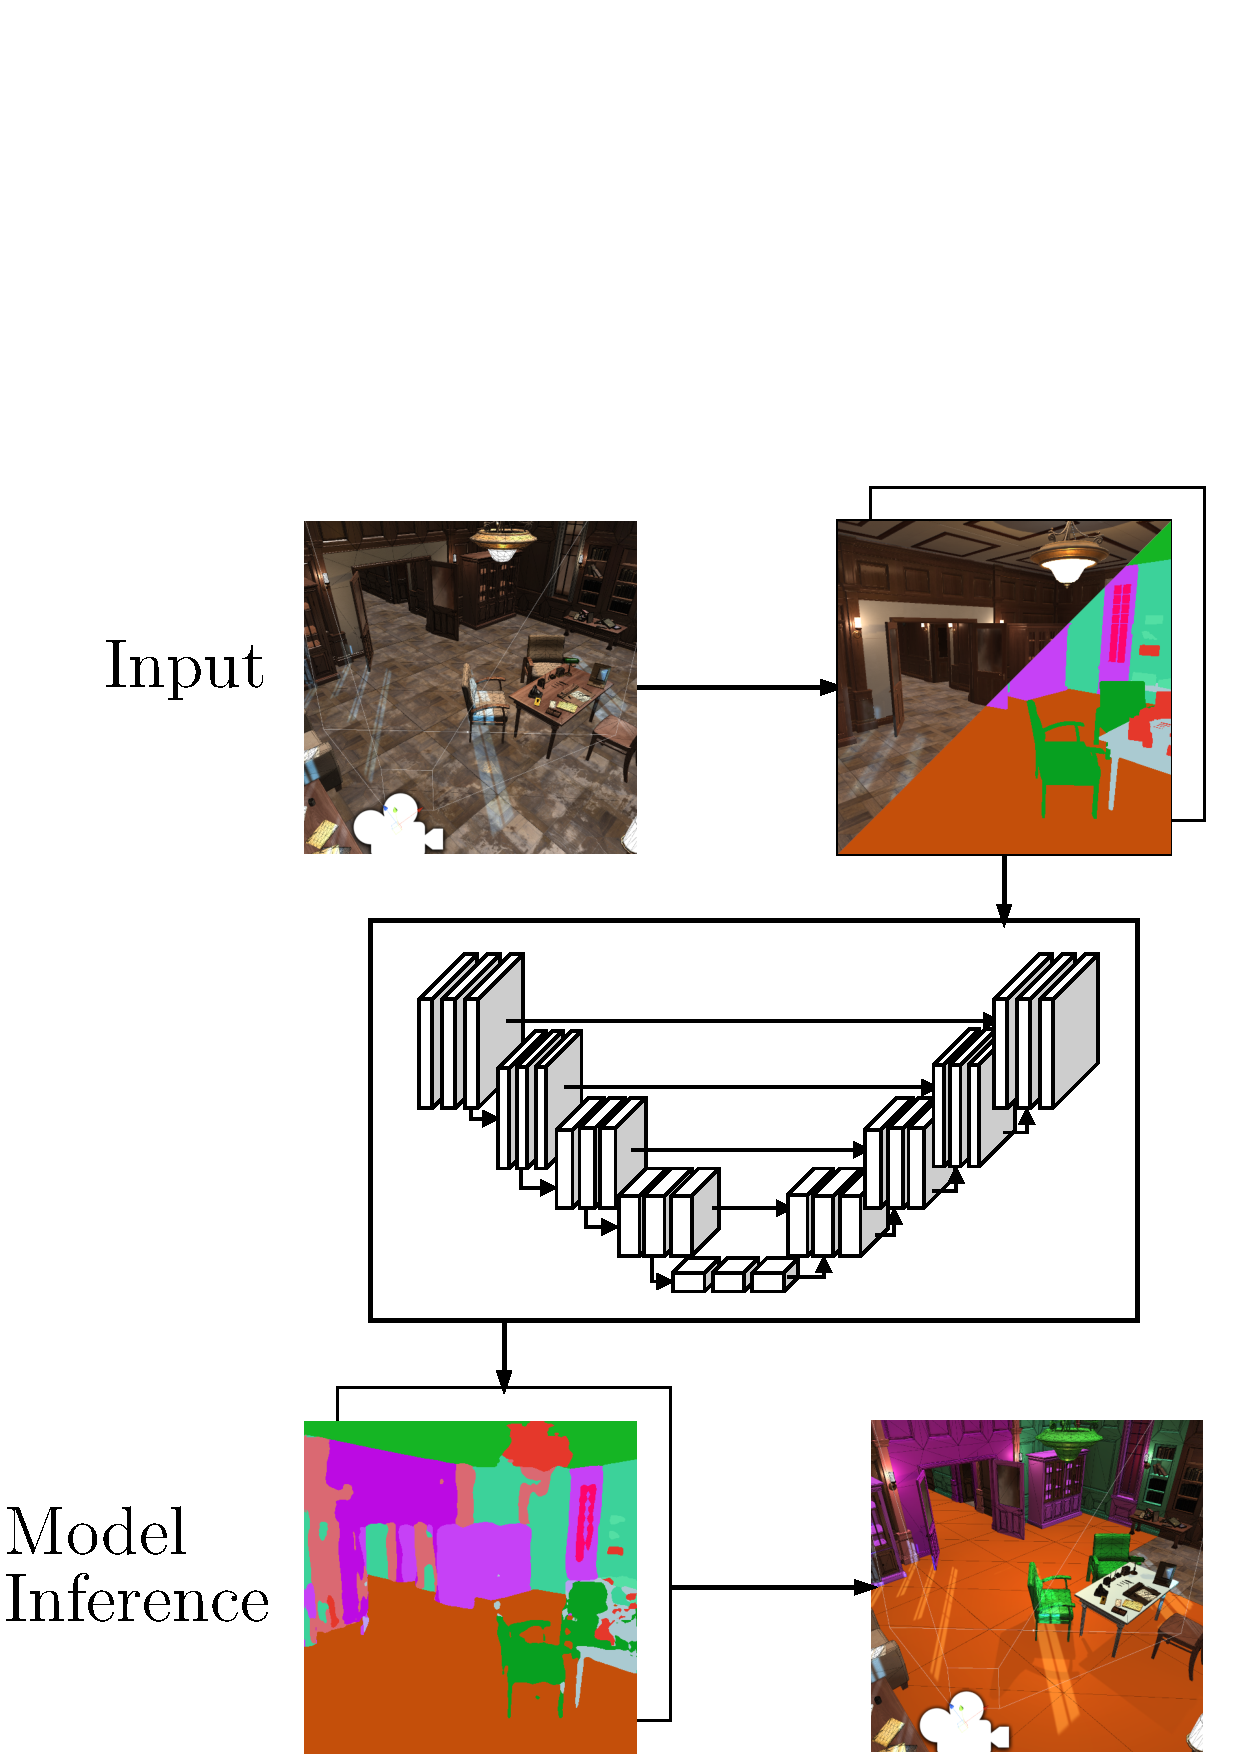
\includegraphics[width=1\linewidth]{camera-pipeline}
    \caption[Camera-based acoustic material tagging system overview]{Overview of the proposed system: given a set of views captured in a VE, a convolutional neural network trained on samples from the test scenes performs semantic segmentation. The predicted semantic maps are then reprojected onto objects in the virtual scene, associating predicted semantic classes with acoustic profiles that are attributed to the scene geometry. Tagged scene geometry provides input to acoustic renderers or physically-based audio engines for sound propagation or synthesis tasks.}
    \label{fig:cog-pipeline}
\end{figure}

\paragraph{Training Phase}
The training phase used an environment with scene geometry tagged with ground truth acoustic materials, reproducing the workflow of audio engineers authoring virtual complex scenes by assigning acoustic properties to scene elements. The system is trained on these scenes by generating a set of camera renders with associated segmentation mapping to the correct pixel-wise category.
\begin{figure}[htbp]
    \centering
    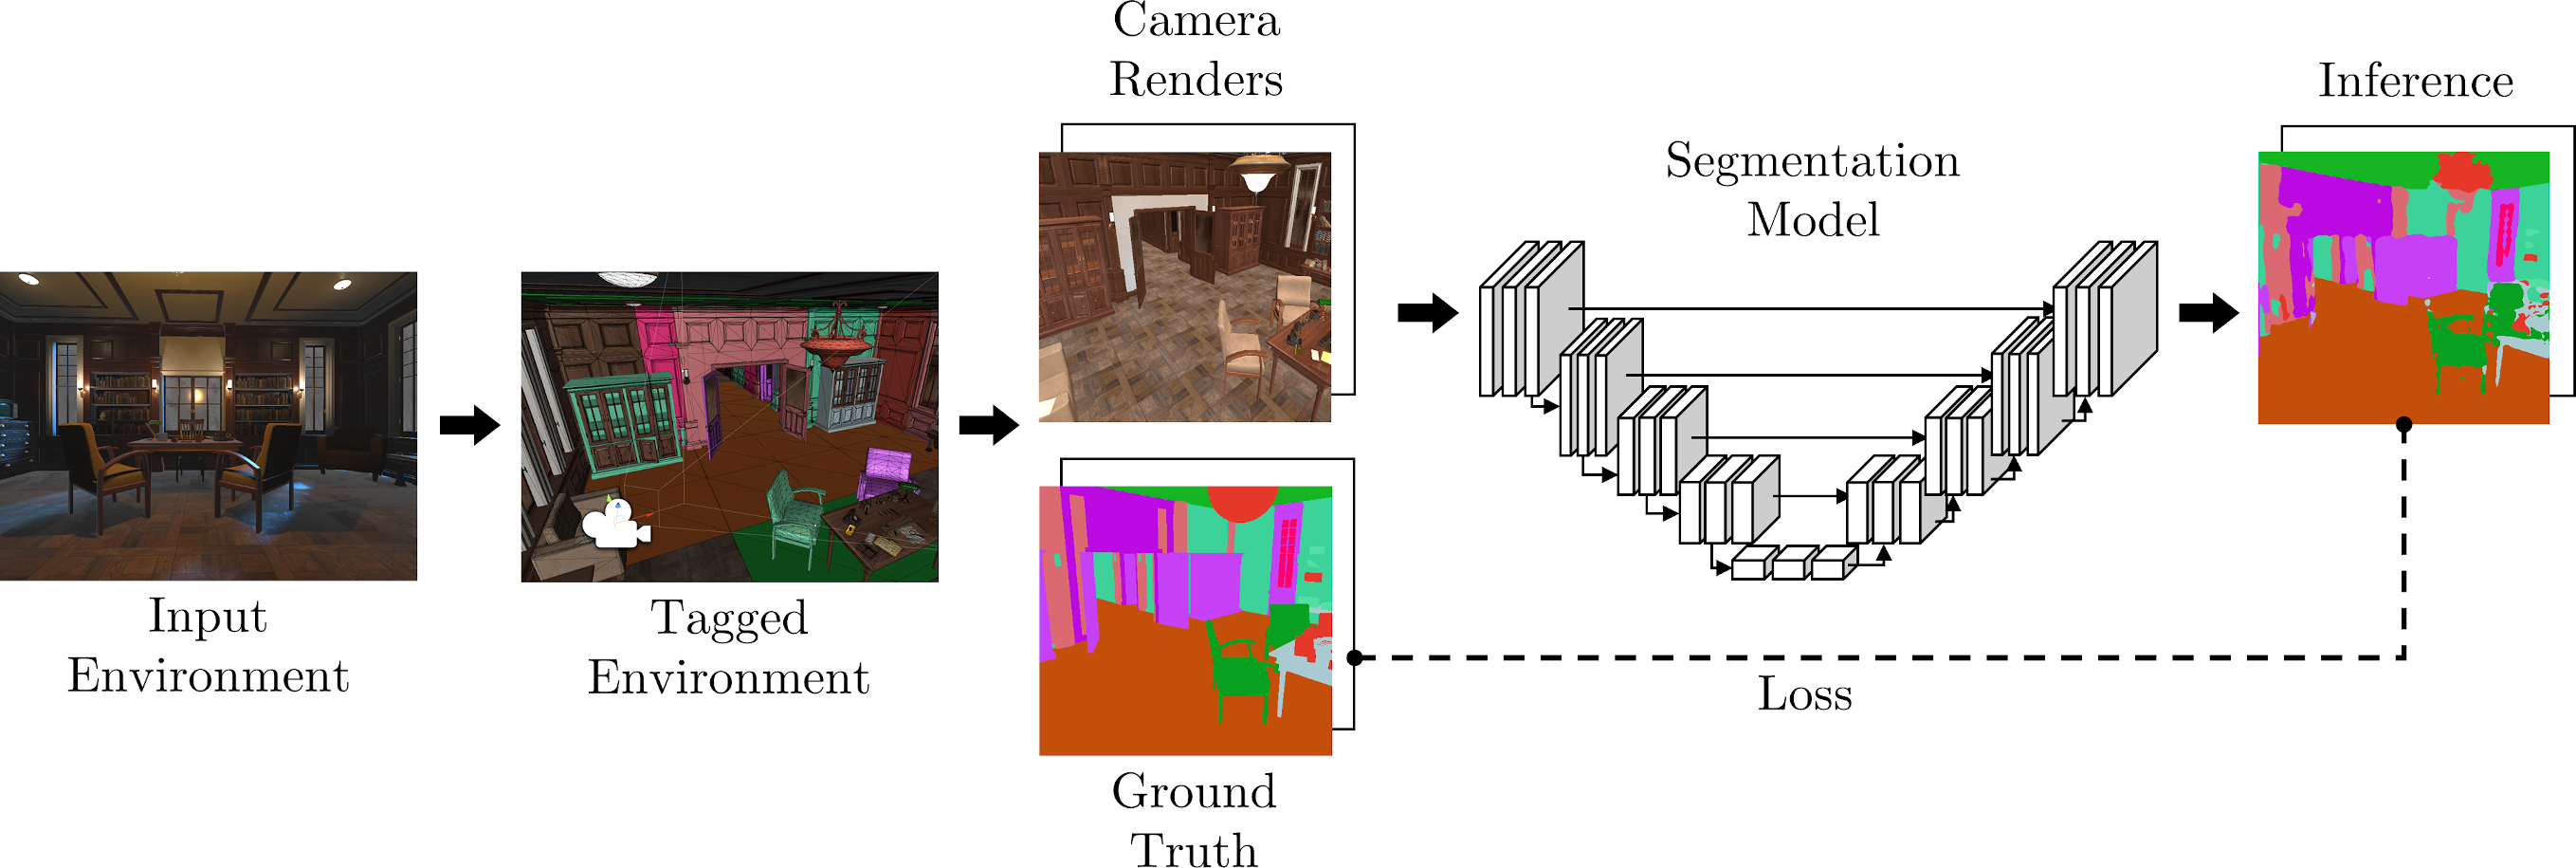
\includegraphics[width=1\linewidth]{cog-pipeline-training}
    \caption[Camera-based acoustic material tagging training]{Training phase of the system pipeline: manual acoustic material tagging is performed on an input environment, generating pairs of camera renders and segmentation maps via ray casting, which are then used to train and evaluate the convolutional neural network.}
    \label{fig:cog-training}
\end{figure}

\paragraph{Inference Phase}
Once the network is fit on the ground truth set, it is deployed to a set of test scenes with no material tags, obtaining camera renders across uniformly spaced camera probes scattered around the walkable space of each scene. The scene is then tagged by predicting segmentation maps and reprojecting acoustic material to virtual geometry.
\begin{figure}[htbp]
    \centering
    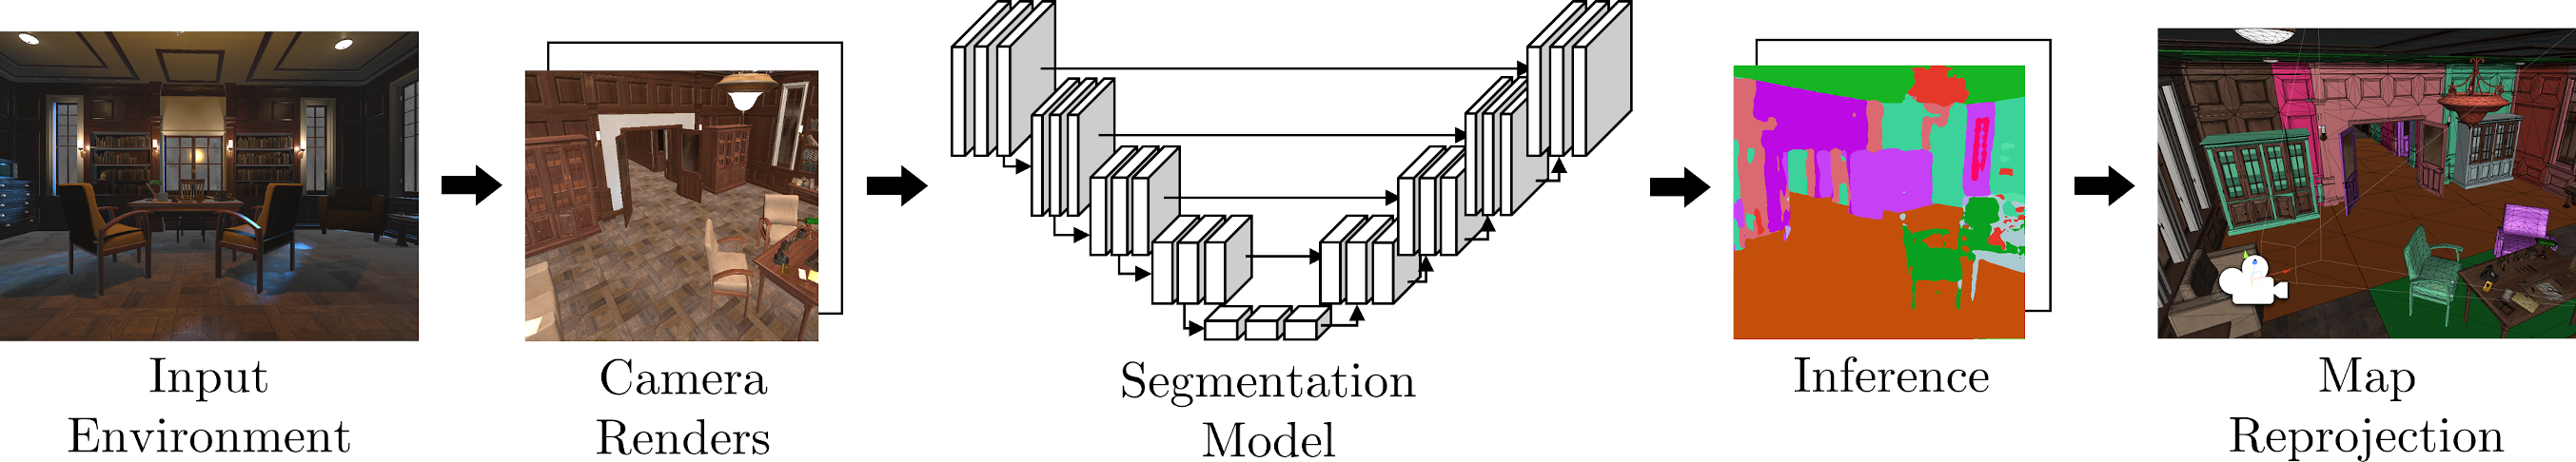
\includegraphics[width=1\linewidth]{cog-pipeline-inference}
    \caption[Camera-based acoustic material tagging inferece]{Inference phase of the system pipeline: camera renders are generated from an input environment, providing input to the convolutional neural network. With camera transformations, segmentation maps generated by the network are used to attribute acoustic properties via semantic class mapping to scene geometry.}
    \label{fig:cog-inference}
\end{figure}

\subsection{Method}\label{sec:mat-method}
Based on advances in scene understanding and the current state of sound renderers, an architecture that enables the process of semantic mesh labelling in complex scenes and associating every category with a frequency-dependent acoustic absorption function is prototyped and tested. Methods based on perceptual metrics should consider only meshes that are relevant to the acoustic environment. Scene understanding methods and inference should be optimised depending on the scene geometry.

\subsubsection{Input}
This method demonstrates the usage of the material tagging system in two scenes: an open, urban environment, \emph{City}, and an indoor wooden room, \emph{Office}. City has $6.3M$ triangles and $8.6M$ vertices. Office has $3.3M$ triangles and $3.8M$ vertices. A set of classes using tables of measured acoustic absorption of construction materials is defined, grouping materials in categories specifying a vector $\alpha$ of absorption coefficient values across an approximated \acrfull{erb} frequency scale ranging from \qty{125}{\Hz} to \qty{4}{\kHz}. Two levels are defined for every major material category in the material database, representing the low and high bounds of mass density $\rho$ in that category. Mass density is a physical property allowing for the acoustic properties of two objects made of the same material to be perceptually distinguishable \citep{giordano2006material}. There are 23 material classes constituted by the two density levels for each of the 11 material categories and an additional class representing ``air''; see Table~\ref{tab:absorption-coeffs}.

\subsubsection{Data Generation}
The data generation pipeline of the material tagging system, implemented in a standard game engine, Unity, uses probe points uniformly scattered across a complex scene to generate labelled data for training and inference purposes. Segmentation masks associated with each view are generated by ray-casting through each point of $C_n$, the \emph{near} camera clipping plane, to $\infty$; see Figure~\ref{fig:cog-reproj-a}.\par
% For this case, we exclude wavelength-based strides to maximise segmentation accuracy.
The areas where rays intersect with $C_f$, the \emph{far} camera clipping plane, are labelled as air; objects that are hit by a ray determine the pixel value of the mask, which points to the corresponding material. The dataset consists of 3500 labelled images with $512\times512$ pixel resolution, split into 3000 training images and 500 validation images.\par
In the City and Office complex scenes, rendered views are generated in different regions of the environments. The different regions delimit spaces for the collection of training and validation data. For each delimited region, sets of points are scattered to cover the walkable space. The camera position is interpolated across points in these sets and rotated between 0 and $2\pi$ along the azimuth and between 0 and $\pi$ along the elevation.\par

\subsubsection{Semantic Segmentation Model}
A convolutional neural network is used to discriminate materials of objects represented in the camera-rendered views. This task is performed with pixel-level semantic segmentation using a ResNet-34-based UNet \citep{ronneberger2015u}. The ResNet backbone offers a topology that is easy to train and has excellent generalisation performance. It also provides a compromise between accuracy and the number of parameters as demonstrated by \cite{he2016deep}.
The model, pre-trained on the ImageNet dataset \citep{deng2009imagenet}, is fine-tuned for 70 epochs minimising focal loss \citep{lin2017focal}. Table~\ref{tab:cog-model} shows the information on the networks trained, including the total number of parameters, $F_{1}$\hyp{}score, Intersection Over Union (IOU), and the number of epochs to obtain fit models.
\begin{table}[htbp]
\caption{CNNs used to produce segmentation maps with the camera-based system, detailing architecture type and performance metrics.}
\centering
\begin{tabular}{lllllll}
\toprule
\textbf{Architecture} & \textbf{Backbone}  & \textbf{Capacity} & \textbf{$\mathbf{F_{1}}$\hyp{}score}   & \textbf{IOU}  & \textbf{Epochs} & \textbf{Loss} \\
\midrule
Unet                  & ResNet-34          & $24.5M$           & $0.51$                                 & $0.58$         & $70$           & $2*10^{-3}$   \\
Unet                  & ResNet-50          & $32.6M$           & $0.54$                                 & $0.47$         & $70$           & $7*10^{-4}$   \\
\bottomrule
\end{tabular}
\label{tab:cog-model}
\end{table}

\subsubsection{Model Inference}
The trained model outputs an $m \times n \times k$ matrix $M$, where $m$ and $n$ are the input image resolution and $k$ is the number of classes. For each pixel, the $k$ channels encode a probability distribution across the classes. Per-pixel classes are determined with the member having the highest presence probability, reducing $M$ to an $m \times n$ matrix where entries encode the semantic class; see Table~\ref{tab:absorption-coeffs}. 
In addition, counts of unique entries in $M$ determine the number of pixels describing the associated material. Scaling based on the distance between a target object and $C_n$ allows material exclusion below a threshold.

\subsubsection{Map Reprojection}
Using the segmented images, meshes are labelled by raycasting through $C_n$ divided in strides, targeting entities within the camera frustum. The process depends on the distance between a target mesh in the game engine and the camera, the stride size is determined by the lowest structural dimension of each mesh, scaled according to its distance to $C_n$. This allows consideration of filtering objects by wavelength, $\lambda = 0.7m$, from the reprojection process. As a result, the material tagging system can dismiss objects that are too small to have a significant impact on the human perception of the soundscape. Through this \acrfull{lod} graduation, scene geometry is simplified, excluding structures having smaller perceptual impacts on the resulting acoustic model and optimising input for sound rendering systems applied to complex scenes.\par
Among the factors affecting the performance and accuracy of acoustical simulation methods is the polygon count of the acoustic \acrshort{ve}, dependent on the complexity of a scene and the presence of detail and small objects. In acoustic environments, smaller structures on surfaces tend to induce scattering of incidental high-frequency waves reflected, and they are neglected by lower frequencies whose wavelength is greater than the structure dimensions. As a consequence, the amplitude of lower frequencies is more likely to be affected by first-order room modes, given by walls and large boundaries, affecting the frequency response of the sound field, resulting in a more noticeable perceptual effect. As opposed to frequencies higher than the Schroeder Frequency, which tend to scatter chaotically \citep{kuttruff2016room, blauert1997spatial}.\par
A study of perceptual optimisations conducted by~\cite{pelzer2010frequency} demonstrates up to 123\% of performance gains in offline and real-time acoustic modelling implementations. Small structures on surfaces can therefore be excluded from modelling processes. Results of this process can be seen in Table~\ref{tab:cog-preliminary-results} (Office, Tagged) where smaller objects than a $\lambda$ of 0.7m do not receive a material tag.\par
% Considering meshes inside the camera frustum, marching cubes algorithms should enable the geometry reduction considering the size of cubes dependent on the wavelength of the lowest frequency \citep{pelzer2010frequency}.
Upon tagging meshes based on pixel-level data extracted from segmentation maps, the confidence value provided by the network when attributing classes to pixels is stored at a mesh level. This is used whenever a subsequent map reprojection overlaps with a previous one, and the same mesh is being reprojected multiple times: in this case, the class with the highest confidence value is used.\par

\begin{figure}
    \centering
    \begin{subfigure}[t]{0.49\textwidth}
       \centering
       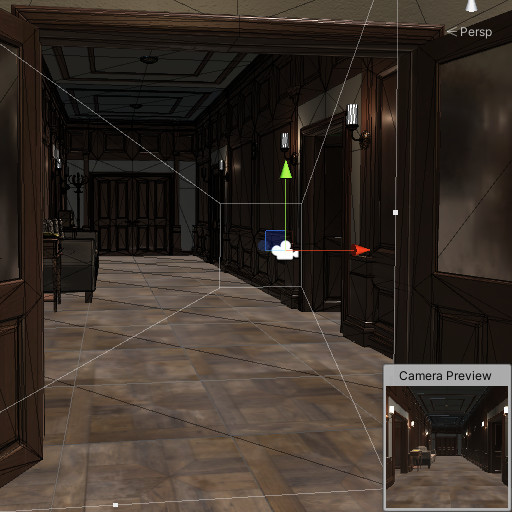
\includegraphics[width=\textwidth]{cog-reproj-a}
       \caption{Input Camera Render}
       \label{fig:cog-reproj-a}
    \end{subfigure}
    \begin{subfigure}[t]{0.49\textwidth}
       \centering
       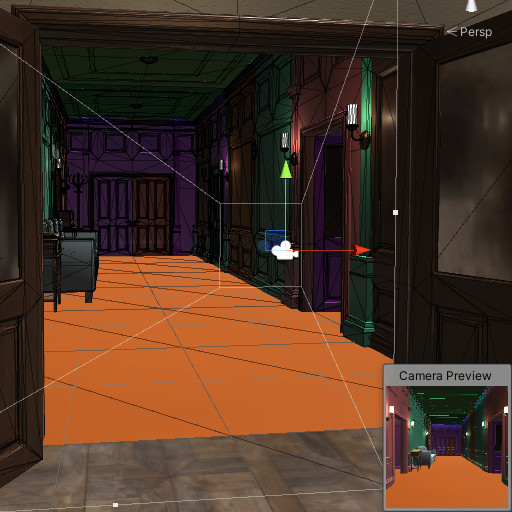
\includegraphics[width=\textwidth]{cog-reproj-b}
       \caption{Re-projected Acoustic Materials}
       \label{fig:cog-reproj-b}
    \end{subfigure}
\caption[Material tagging segmentation reprojection system]{Map Reprojection performed on an input camera render: based on a predicted segmentation map, acoustic materials determined by pixel-wise semantic information are re-projected onto scene objects captured by the camera.}
\label{fig:cog-reprojection}
\end{figure}

\subsection{Acoustic Materials}
\begin{table}
    \def\widthspark{120pt}
    \centering
    \caption[Acoustic material definitions]{Common acoustic absorption coefficients with ranges (low-high) of $\alpha$ absorption characteristics across the frequency bands for those material types. It should be noted that these are regressions and averages of generally adopted materials and existing measurement tables; realistic or surveying acoustic simulations should adopt absorption measurements of real materials.}
    \begin{tabular}{lll}
    \toprule
    \textbf{Material}                  & \textbf{Low $\alpha$}                                                              & \textbf{High $\alpha$}                                                               \\ \midrule
    Glass and glazing                  & 
\includegraphics[width=\widthspark]{sparklines/glass and glazing_low}               & 
\includegraphics[width=\widthspark]{sparklines/glass and glazing_high}               \\ 
    Masonry walls                      & 
\includegraphics[width=\widthspark]{sparklines/masonry walls_low}                   & 
\includegraphics[width=\widthspark]{sparklines/masonry walls_high}                   \\ 
    Stud-work \& lightweight walls     & 
\includegraphics[width=\widthspark]{sparklines/studwork and lightweight walls_low}  & 
\includegraphics[width=\widthspark]{sparklines/studwork and lightweight walls_high}  \\ 
    Wood \& wood panelling             & 
\includegraphics[width=\widthspark]{sparklines/wood and wood panelling_low}         & 
\includegraphics[width=\widthspark]{sparklines/wood and wood panelling_high}         \\ 
    Floors                             & 
\includegraphics[width=\widthspark]{sparklines/floors_low}                          & 
\includegraphics[width=\widthspark]{sparklines/floors_high}                          \\ 
    Panels \& doors                    & 
\includegraphics[width=\widthspark]{sparklines/panels and doors_low}                & 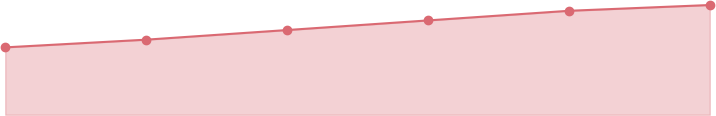
\includegraphics[width=\widthspark]{sparklines/panels and doors_high}                \\ 
    Other                              & 
\includegraphics[width=\widthspark]{sparklines/other_low}                           & 
\includegraphics[width=\widthspark]{sparklines/other_high}                           \\ 
    Wall treatments \& construction    & 
\includegraphics[width=\widthspark]{sparklines/wall treatments & constructions_low} & 
\includegraphics[width=\widthspark]{sparklines/wall treatments & constructions_high} \\ 
    Ceilings                           & 
\includegraphics[width=\widthspark]{sparklines/ceilings_low}                        & 
\includegraphics[width=\widthspark]{sparklines/ceilings_high}                        \\ 
    Mineral wool \& foams              & 
\includegraphics[width=\widthspark]{sparklines/mineral wool and foams_low}          & 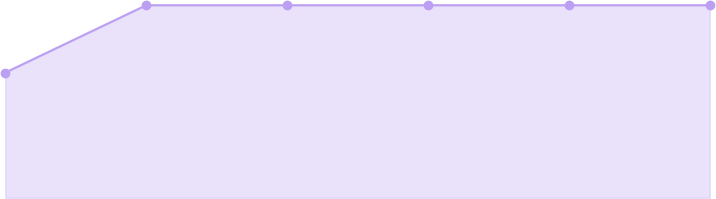
\includegraphics[width=\widthspark]{sparklines/mineral wool and foams_high}          \\ 
    Audience \& seating                & 
\includegraphics[width=\widthspark]{sparklines/audience and seating_low}            & 
\includegraphics[width=\widthspark]{sparklines/audience and seating_high}            \\ 
    \bottomrule
    \end{tabular}\label{tab:absorption-coeffs}
\end{table}
Table~\ref{tab:absorption-coeffs} shows acoustic material definitions for the camera-based system. In light of the introduction to materials in Section~\ref{sec:bg-materials}, acoustic materials in the experiments illustrated in this thesis are defined as a set of absorption coefficients mapped to the scene geometry.\par
Each entry in the table has two variants for a given semantic material: a low and high absorption variant. This categorisation allows the reduction of dimensionality of standard acoustic material databases\footnote{\url{https://odeon.dk/downloads/materials/}} whilst keeping the differentiation between instances of the same semantic material class.

\subsubsection{Evaluation}
An acoustic renderer is used to test the validity of this method by producing auralisations of Office. City is excluded because of its computationally expensive scene complexity. The evaluation uses a state-of-the-art acoustic renderer proposed by \cite{raghuvanshi2014parametric}, Project Acoustics. It integrates into Unity, to generate a model of the acoustic environment using the parametric wavefield coding technique to compute effects between sources and receivers through wave-based acoustic rendering. The renderer determines per-mesh absorption information based on the texture meta-data as per default behaviour. A sound source and listener are placed at human height in the scene; the listener captures a $30s$ chirp signal sweeping logarithmically from \qty{20}{\Hz} to \qty{20}{\kHz} emitted by the sound source to measure an \acrshort{ir}. Maintaining the same settings and positions of source and listener, the procedure of supplying meshes and absorption information inferred by the system is repeated, generating the Tagged data. The evaluation compares the two IRs generated by the former (Default) and the latter acoustic model (Tagged) through comparisons of frequency responses; see Table~\ref{tab:cog-preliminary-results}.

\subsection{Results}
The model inference takes an average of $400 ms$ and the re-projection process takes an average of $96ms$. These figures are quoted per camera probe that is used to generate acoustic labels for surfaces in the scene. Images to be inferred are of a fixed size from the scene frame buffer, $512 \times 512$ pixels. The time taken for inference is largely invariant to typical scene complexities such as shape, polygon count, materials etc. The Office scene requires 12 probes to completely tag the environment, requiring $\sim$6s to complete the tagging process. The City scene shown has extra complexity and requires the use of solutions to the Art Gallery problem to deduce the minimum number of probes to cover the space and tag all objects.\par
As shown in Table~\ref{tab:absorption-coeffs}, acoustic properties can be associated with geometry in the scene, and can be tagged from camera probes. These materials are used in an acoustic rendering process, either directly in audio engines or external offline acoustic renderers. This can result in more realistic aural spatialisation, using IRs to encode early and late reflections.\par
Currently, this camera-based approach works by providing inference for camera views within the scene. These camera views are manually placed and would need to be placed in many positions in order to tag materials accurately for the entire scene. The process still requires a human-in-the-loop and needs to be addressed to ensure the goal of having the system as an end-to-end autonomous vision-based material tagging system.\par
To extrapolate materials tagged to the entire scene, solutions to the Art Gallery problem would optimise the number of predictions required \cite{devadoss2011discrete, bajuelos2008optimizing}. Considering the polygons encapsulating the walkable space $W$ of a scene, minimum vertex guard algorithms suggest that $\floor*{n/3}$, where $n$ indicates the total vertices of $W$, is the least number of positions from where the entire scene can be seen. Based on the depth of the camera, additional intermediate positions $\textbf{p}$ might be needed to accurately represent objects, this also depends on the number of pixels per object allowing the the neural network to infer materials from the set of camera views that facilitate the whole scene to be visible. For each camera probe position, rotation steps are needed to ensure that all points of $W$ are inside the camera frustum. For an omnidirectional camera probe, these rotation steps $\textbf{r}_\theta$ for azimuthal steps and $\textbf{r}_\phi$ for elevation steps should cover the space in $2\pi$ azimuth and $\pi$ elevation. The resulting complexity of the material tagging process for the scene would then be determined by $O(\floor*{n/3} + \textbf{p} + \textbf{r}_\theta + \textbf{r}_\phi)$.
\begin{landscape}
\begin{table}[]
\def\cogimsw{0.19\textwidth}
\centering
\caption{Results from tests conducted on the City and Office complex scenes by applied the camera-based acoustic material tagging system.}
\begin{tabular}{@{}lllllll@{}}
\toprule
Render & Input & Segmented & Tagged & Render & Input & Segmented \\ \midrule
\multicolumn{1}{c}{}  & \multicolumn{3}{c}{Office} & \multicolumn{3}{c}{City} \\
\multicolumn{1}{c}{A} &  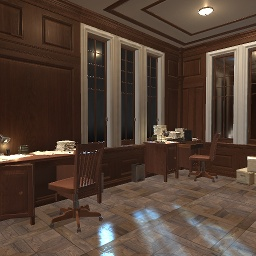
\includegraphics[width=\cogimsw]{Office_A_original} & 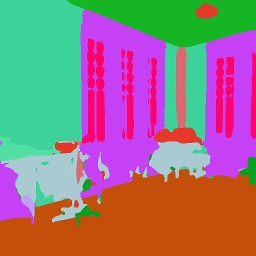
\includegraphics[width=\cogimsw]{Office_A_segmented} & 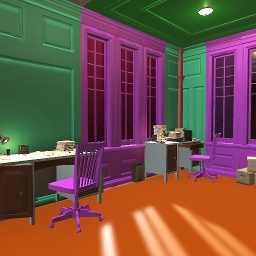
\includegraphics[width=\cogimsw]{Office_A_tagged} & 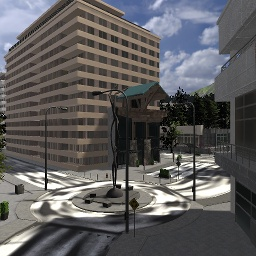
\includegraphics[width=\cogimsw]{City_A_original} & 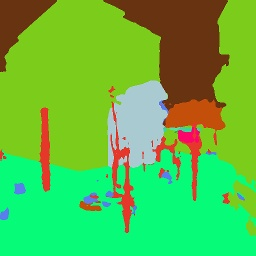
\includegraphics[width=\cogimsw]{City_A_segmented} & 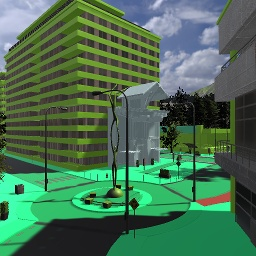
\includegraphics[width=\cogimsw]{City_A_tagged} \\
B & 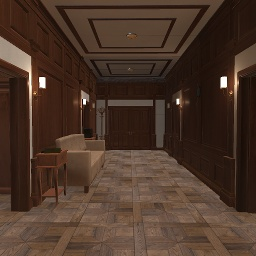
\includegraphics[width=\cogimsw]{Office_B_original} & 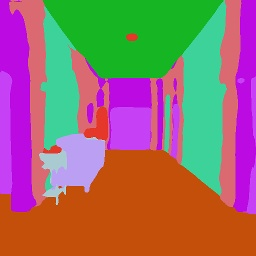
\includegraphics[width=\cogimsw]{Office_B_segmented} & 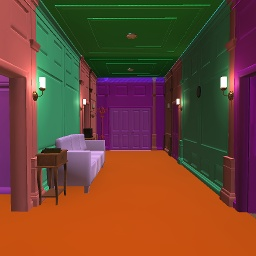
\includegraphics[width=\cogimsw]{Office_B_tagged} & 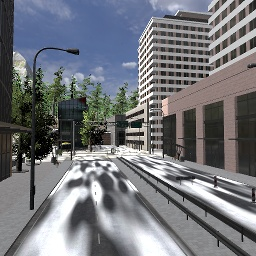
\includegraphics[width=\cogimsw]{City_B_original} & 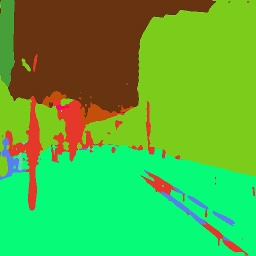
\includegraphics[width=\cogimsw]{City_B_segmented} & 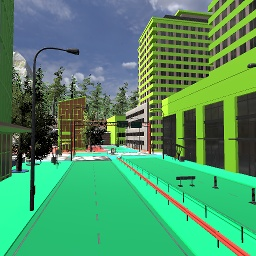
\includegraphics[width=\cogimsw]{City_B_tagged} \\
C & 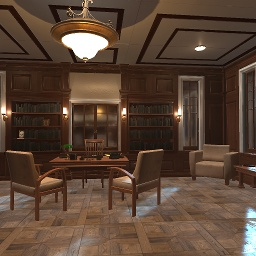
\includegraphics[width=\cogimsw]{Office_C_original} & 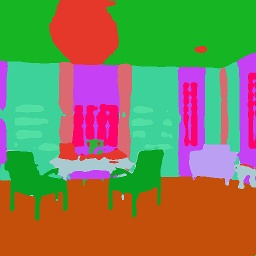
\includegraphics[width=\cogimsw]{Office_C_segmented} & 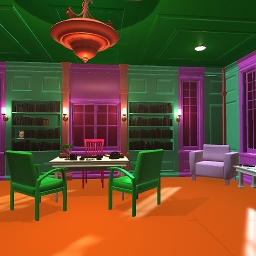
\includegraphics[width=\cogimsw]{Office_C_tagged} & 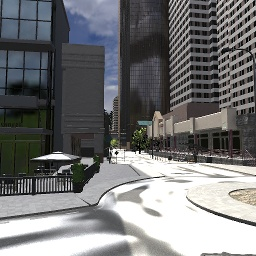
\includegraphics[width=\cogimsw]{City_C_original} & 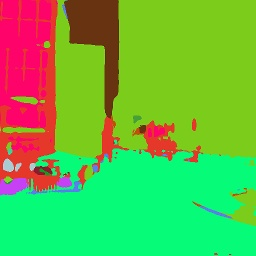
\includegraphics[width=\cogimsw]{City_C_segmented} & 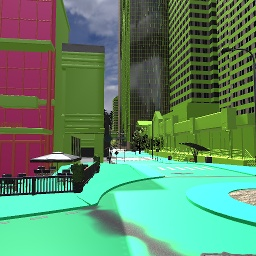
\includegraphics[width=\cogimsw]{City_C_tagged} \\
D & 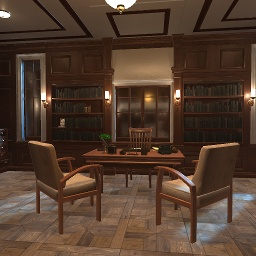
\includegraphics[width=\cogimsw]{Office_D_original} & 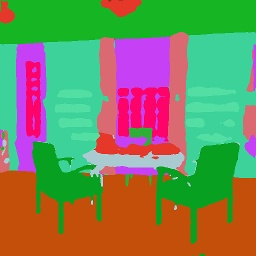
\includegraphics[width=\cogimsw]{Office_D_segmented} & 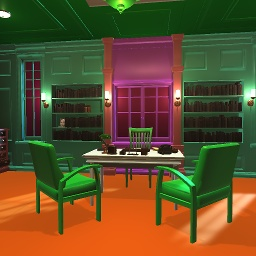
\includegraphics[width=\cogimsw]{Office_D_tagged} & 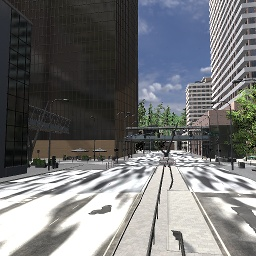
\includegraphics[width=\cogimsw]{City_D_original} & 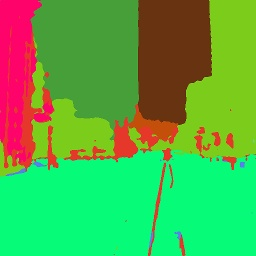
\includegraphics[width=\cogimsw]{City_D_segmented} & \includegraphics[width=\cogimsw]{City_D_tagged} \\
\multicolumn{1}{l}{legend} & \multicolumn{6}{c}{legend}
\end{tabular}
\label{tab:cog-preliminary-results}
\end{table}
\end{landscape}

\subsection{Discussion}
Acoustic modelling and audio rendering methods can benefit from research and development of computer vision methods. The current status of this method does not fully eliminate the human-in-the-loop; however, it can generalise and operate on large sets of complex scenes. As a result, artistic and creative workflows for level design can benefit from an automated material tagging system that is agnostic of scene complexity and allows for easy integration of wave-based acoustic renderers.
The next steps should include the development of a generalised system to perform material tagging in complex scenes, considering optimisation methods to allow the inference of entire scenes automatically with the minimal set of camera probes to consistently tag every acoustically congruent object that is contributory to the \acrshort{ve}.\par
One crucial advantage of a camera-based acoustic material recognition system is the potential to tailor the recognition of materials based on their appearance to a defined ecosystem of material appearances expressed by a set of virtual environments. Although this aspect contrasts the goal of \acrshort{cnn} of providing generalisable models, it addresses the problem of the large variance found in visual features of materials by constraining the network within a range of material appearances that interest VE designers. Resembling workflows common in \acrfullpl{naf} \citep{mildenhall2020nerf}, game designers or VE artists would need to provide exemplary scenes tagged with a customisable set of acoustic and semantic materials to the camera-based system, enabling acoustic material tagging of unseen or novel scenes sharing the same nature. With the rising availability of computational resources allocated to rendering VEs, performing a forward pass with a ResNet50 CNN \citep{he2016deep} is becoming feasible at runtime, unlocking the potential for online sound propagation on dynamic scenes.\par
% % Case for tailoring material recognition to ecosystems of materials
% Case for artistic material tags

\section{Texture-based Acoustic Material Tagging}\label{sec:texture-tagging}
In this Section, a novel architecture for tagging acoustic material in virtual environments, abstracting away from camera-based systems, is developed and tested. By working on virtual reconstructions of complex scenes, this approach is agnostic of the technology and architecture of the target platform. Despite the significant progress made in sound propagation over the last decades, there are still many limitations in simulations for indoor and outdoor environments due to the complexity of the factors that describe a wavefield \citep{liu2020sound}. The texture-based system considers the discussion around the camera approach and expands towards:
\begin{itemize}
    \item a more efficient application of acoustic rendering to virtual environments;
    \item a novel architecture for recognising materials from textured meshes in complex scenes, reducing the need for manual tagging of acoustic materials and eliminating the needs for camera-based workflows; 
    \item an objective evaluation of the architecture conducted on a virtual reconstruction of a real conference room.
\end{itemize}

\subsection{Method}
The texture-based system is presented as a method for processing scene geometry, generating input for sound rendering pipelines by predicting materials of objects composing complex scenes. A system overview shown in Figures~\ref{fig:texture-tagging-training} and~\ref{fig:texture-tagging-inference} illustrates how visual representations of the environment map to acoustic data used by sound renderers to model sound propagation in a scene. Similarly to the camera-based approach, there is a \emph{training} and \emph{inference} phase.\par
In summary, the unwrapped texture of each mesh in the scene geometry provides representations of their materials, which provide input for a convolutional neural network. Based on features extracted from textures, the network recognises different material labels in textures and maps them to acoustic data from a database, expressed as acoustic materials.

\subsubsection{Material Recognition}
According to \cite{schwartz2019recognizing}, small image patches contain enough information to distinguish materials and hence, this method decomposes input image textures into small image patches.
\subsubsection{Training}
\begin{figure}[htbp]
    \centering
    \includegraphics[width=1\linewidth]{chi-training}
    \caption[Texture-based material recognition system --- training phase]{Overview of the texture-based system set up for the \emph{training} phase: a network extracts features from superpixel data, obtained from image textures from scene objects in virtual environments. Extracted features are used to classify semantic materials. The system trains on a large dataset of annotated image patches gathered from in-the-wild photographs of real surfaces.}
    \label{fig:texture-tagging-training}
\end{figure}
The training pipeline determines the visual material space by applying transfer learning to the OpenSurfaces dataset \citep{bell2013opensurfaces}, which comprises 36 classes of surface photographs. To do so, a SLIC superpixel segmentation algorithm \citep{slic6205760} segments input surface photographs into a set of superpixel labels, determining regions correlated with boundaries of objects. These resulting superpixel labels are then used to generate rectified image patches encapsulating their contours through edge detection, adopting~\cite{ding2001canny}'s method.
Rectified image patches provide input to a ResNet50 \citep{he2016deep}, used as a feature extractor for a classification network using a standard fully connected layer to predict class labels based on embeddings of $32\times32$ pixel resolution input patches. The network trains the network on \num{13677819} input patches, composing a train set of about 9.1M images and an evaluation set of about 4.5M, adopting the standard Adam optimiser \citep{kingma2014adam} to update the weights initialised from the ImageNet dataset \citep{deng2009imagenet}. The model usually converges in 45 epochs with a training and validation accuracy of about $0.94$ and $0.83$ respectively. 

\subsubsection{Inference}
\begin{figure}[htbp]
    \centering
    \includegraphics[width=1\linewidth]{chi-inference}
    \caption[Texture-based material recognition system --- inference phase]{Overview of the texture-based system set up for the \emph{inferece} phase: textures mapped to meshes representing scene objects are decomposed into image patches using SLIC superpixel segmentation. A trained classifier extracts features from image patches and generates acoustic materials, which are then mapped against geometry representing the given scene object.}
    \label{fig:texture-tagging-inference}
\end{figure}
During the \emph{inference} phase, the set of textured meshes in given a scene is used to unwrap textures as images, prividing input to the trained network to recognise acoustic materials; see Figure~\ref{fig:texture-tagging-inference}. The trained ResNet50 extracts features from input image textures in complex scenes, whose embeddings enable the classifier to predict class labels associated with each input superpixels. The most frequent prediction maps to an acoustic measurement database, defining the output acoustic material. On average, the classifier takes $11.2s$ to determine the acoustic material for a given texture, see Figure~\ref{fig:slic-generation}, divided in $3.8s$ for generating rectified patches and $7.3s$ to extract features and compute the mapping. The transparency information contained in the mesh texture is preserved, allowing the network to dismiss image patches that do not contain visual features as demonstrated in Figure~\ref{fig:slic-labels}.

\subsubsection{Acoustic Material Mapping}
Material labels inferred from textures are associated with acoustic measurements of absorption coefficients. For every label, a one-to-many mapping group measurements of the given material. Following the methodology developed by~\cite{kim2020acoustic}, the system uses median frequency-dependent values to determine acoustic absorption, defining acoustic materials. A single acoustic material maps to each given mesh, associating a vector of acoustic absorption coefficients to its triangles, determining the overall acoustic mapping accuracy to depend upon the mesh separation of the scene geometry. In the example texture shown in Figure~\ref{fig:slic-generation}, ``Tile'' defines the acoustic material, as per predictions shown in Figure~\ref{fig:slic-label-inference}.
\begin{figure}[htbp]
    \centering
    \begin{subfigure}[t]{0.49\textwidth}
       \centering
       \includegraphics[width=\textwidth]{slic-input-texture}
       \caption{Input Texture}
       \label{fig:slic-input-texture}
    \end{subfigure}
    \begin{subfigure}[t]{0.49\textwidth}
       \centering
       \includegraphics[width=\textwidth]{slic-texture}
       \caption{SLIC Superpixels}
       \label{fig:slic-labels}
    \end{subfigure}
\caption[SLIC superpixel computation on a texture]{SLIC Superpixel computation on real texture from a virtual reconstruction of a conference room.}
\label{fig:slic-generation}
\end{figure}%
\begin{figure}[htbp]
    \centering
    \includegraphics[width=1\linewidth]{slic_labels}
    \caption[Superpixel algorithm used to generate image patches]{Predicted Class labels from input image patches computed from the texture shown in Figure~\ref{fig:slic-generation}.}
    \label{fig:slic-label-inference}
\end{figure}


\subsection{Evaluation}
The texture-based acoustic material tagging system is evaluated by deploying it to a real-world scene, using a state-of-the-art \acrshort{ga} acoustic renderer. In order to compare acoustic models estimated with state-of-the-art wave-based audio renderers, testing whether the proposed system for the automatic tagging of scene geometry has a significant impact on the resulting acoustic model. The experimental evaluation uses a real environment as a benchmark for testing how predicted models express acoustic parameters of measurable space.

\subsubsection{Scene Geometry Reconstruction}
Wavefields are simulated, via the wave-based renderer, from a real conference room that is $3.53m$ deep, $2.84m$ wide and $3.51m$ tall. Theoretically, the dimensions determine a Schroeder frequency of $261Hz$. The room geometry is composed of $2.9M$ of triangles and $6.6M$ vertices and is handled by the Unity game engine.
The geometry of a conference room is reconstructed to deploy the proposed system in a real environment and conduct the subsequent subjective experimental evaluation. The reconstruction process adopts a LiDAR scanner, the FARO Focus\textsuperscript{3D} X300\footnote{\url{https://www.faro.com/en/Products/Hardware/Focus-Laser-Scanners}}, to capture several point clouds scans of the room across 8 positions: 4 position points for each corner of the room at $1m$ height and 4 additional positions at $0.2m$ height to capture furniture and materials from different angles and enhance the spatial resolution. The reconstructed mesh obtained by registering and triangulating the point clouds using the FARO SCENE Software~\footnote{\url{https://www.faro.com/en/Products/Software/SCENE-Software}} is then manually segmented using Blender\footnote{\url{https://www.blender.org/}}, to ensure that a separate textured mesh represents every scene object.
\begin{figure}
    \centering
    \begin{subfigure}[t]{0.49\textwidth}
       \centering
       \includegraphics[width=\textwidth]{environment}
       \caption{Real space}
       \label{fig:chi-input-env}
    \end{subfigure}
    \begin{subfigure}[t]{0.49\textwidth}
       \centering
       \includegraphics[width=\textwidth]{reconstructed}
       \caption{Reconstructed environment}
       \label{fig:chi-reconstructed-env}
    \end{subfigure}
\caption[Texture-based system evaluation --- environment reconstruction process]{}
\label{fig:chi-scanning}
\end{figure}

\subsubsection{Soundfield Measurements}
The experimental evaluation compares simulated wavefields generated from the reconstructed environment to a sample measurement of the real counterpart's wavefield. The evaluation compares wavefields using \acrshort{rir} to describe acoustic properties dependent on geometry and materials surrounding a sound transmission between a source and a listener \citep{stan2002comparison}. The soundfield measurement process captures the environments' acoustic characteristics emitting and recording an exponentially swept sine, ranging from $20Hz$ to $20kHz$, emitted from a speaker and received by a microphone. The speaker-microphone position pair is reproduced in the virtual reconstruction of the space using a virtual sound source and receiver, see Figure~\ref{fig:chi-scanning}. Applying inverse filtering, the \acrshortpl{rir} is recovered from the captured signal \citep{holters2009impulse}. Due to the objective nature of the evaluation, characteristics of human listeners are not considered by the evaluation, hence omnidirectional sources and receivers are used.\par
In the conference room, a public address system, the dB Technologies ES 1002\footnote{\url{https://www.dbtechnologies.com/en/products/es/es-1002/}}, emitted the exponentially swept sine converted from a laptop using an Audient ID14\footnote{\url{https://audient.com/products/audio-interfaces/id14/overview/}} DAC and ADC, which captured the signal back through an omnidirectional, flat-frequency response soundfield measurement microphone, the Earthwork M30\footnote{\url{https://earthworksaudio.com/measurement-microphones/m30/}}.
Steam Audio \citep{audio2020git} is used as a standard acoustic renderer to simulate wavefields from the reconstructed environment. This allows the synthesis of wavefields based on acoustic geometry, considering absorption coefficients expressed across three frequency bands: low, medium and high. All simulations share the same resolution of 65536 and 16384 direct and secondary rays, respectively, with 256 bounces off solid geometry. With the same setup, the evaluation synthesiss three wavefields with different acoustic materials: the \emph{generic} with a single acoustic material for the entire scene geometry; the \emph{tagged}, with acoustic materials assigned through manual material tagging; and \emph{ours}, using the proposed automatic tagging.

\subsubsection{Perceptual test}
The evaluation design also considers subjective factors by conducting a perceptual comparison between simulated wavefields at the same positions of source and listener, see Figure~\ref{fig:chi-scanning}, by using an automated perceptual metric learned on subjects’ responses \cite{manocha2020differentiable}. The metric consists of a 14-layer deep neural network with filters trained on features extracted from paired input audio samples; it expresses a distance $D(x_{ref}, x_{per})$ between two input signals, where $x_{ref}$ is a reference signal, and $x_{per}$ is a perturbated signal. The function $D$ considers factors including reverb and the ratio between direct and reverberated signal. The test evaluates whether the metric expresses a closer perceptual distance between the measured ground truth and the synthesised wavefields, by convolving the \acrshortpl{rir} to samples from the evaluation subset of a database for acoustic scene classification, which comprises 15 different acoustic environments, generating a total of 18 minutes of audio over 1620 $N$ samples \citep{mesaros2016tut}. The learned metric determines the distance between the ground truth convolutions and each of the relative simulated \acrshortpl{rir}: for each audio sample $k$ in $N$, the evaluation determines perceptual distances $D(x_{ref, k}, x_{per_i, k}~\forall~i \in \{generic, tagged, ours\})$, where $ref$ and $per_i$ are the measured and simulated RIRs.

\subsection{Evaluation Results}
%TODO
The evaluation compares an artistic material tag, \emph{tagged}, which assigns acoustic geometry in the scene by applying the methodology used by game designers when tagging scenes; a \emph{generic} tag, where all meshes map to a single acoustic material that expresses $0.1\alpha$ acoustic absorption coefficient across all frequency bands; and finally, \emph{predicted}, having meshes mapping to acoustic materials inferred by the proposed system. For each acoustic material, the sound renderer assigns its acoustic absorption coefficients to all triangles of the corresponding mesh.
The system takes around 7 minutes to compute acoustic materials for the 38 meshes composing the reconstructed environment.
Figures~\ref{fig:texture-testing-rirs}, and~\ref{fig:texture-testing-spectograms} show the magnitude of early reflections for each acoustic simulation. Note that the ground truth shows distortion errors caused by the constant noise floor of $-55dB$ at the time of measurement. The \emph{predicted} acoustic simulation marks the fastest decay in reverberation energy with a $T_{60}$ of \qty{0.44}{\second}, computed parameterising the RIRs according to \cite{lima_RIR_Parameters}. The ground truth is \qty{0.43}{\second}, and generic and tagged are respectively $0.054s$ and $0.073$.

\begin{figure}[htbp]%
    \centering
    \includegraphics[width=1\textwidth]{rir-texture-testing}%
    \caption[Texture-based system testing IR results --- time domain]{Measured impulse responses from measurements shown as normalised direct energy of reflections in function of time $h(t)$.  Energy functions of measured impulse responses, shown in the time domain where the horizontal axis indicates time, and the vertical axis indicates magnitude of reflection energy from 0 to 1.}%
    \label{fig:texture-testing-rirs}%
\end{figure}%

\begin{figure}[htbp]%
    \centering
    \includegraphics[width=1\textwidth]{rir-texture-testing-spectrograms}%
    \caption[Texture-based system testing IR results --- frequency domain]{Spectrograms, computed with triangular windows, showing decay of early reflections across a logarithmic frequency range from $10^2Hz$ to $10kHz$. 
        Spectrograms comparing the frequency content of measured and simulated impulse responses. The impulse response generated with the proposed system maintains more energy over time.}%
    \label{fig:texture-testing-spectograms}%
\end{figure}%

\begin{table}[htbp]%
    \centering
    \caption[Texture-based material recognition correlation scores]{A table showing Pearson $r$ scores for correlation measuring similarity across audio stimuli from simulated soundfields using different acoustic material sets. Generic acoustic materials are defined as $0.1$ acoustic absorption across all frequency bands. Tagged materials are manually assigned, and Predicted materials are inferred from the texture-based material recognition system}%
    \begin{tabular}{lllll}%
    \toprule
              &                     & Generic & Tagged        & Predicted  \\ \midrule 
    Generic   & $r$                 & 1       & 0.85          & 0.854 \\
              & Sig. (2-tailed)     &         & 0             & 0     \\ 
    Tagged    & $r$                 & 0.85    & 1             & 0.96  \\
              & Sig. (2-tailed)     & 0       &               & 0     \\ 
    Predicted & $r$                 & 0.854   & \textbf{0.96} & 1     \\
              & Sig. (2-tailed)     & 0       & \textbf{0}    &       \\ \bottomrule
    \end{tabular}%
    \label{tab:chi-perceptual-distance}%
\end{table}%
The perceptual metric between the measured ground truth and the synthesised wavefields yields three variables describing 1620 pairwise distances between the measured and synthesised RIRs, see Table~\ref{tab:chi-perceptual-distance}. Given the test conditions, the correlation test uses Pearson \textit{r} scores to measure the relationship between RIRs with different acoustic geometry.


\section{Proof of Concept Demonstration}
A proof of concept implementation is designed to work on real-world scenes, gathering insights into the performance of the proposed material tagging prototypes in attributing acoustic properties to segments of the scene geometry of a given environment expressed as a set of triangulated meshes. The design focuses on scenes scanned with space reconstruction techniques applied to real environments, emulating space reconstruction paradigms often adopted by AR HMDs.\par
The design prototype uses standard space-sensing cameras to produce triangulated meshes from a set of real environments. These virtual reconstructions are then processed, segmenting the scene of each environment by generating portions of scene geometry into a set of semantically meaningful sub-meshes expressing elements of the scene. Submeshes are tagged with acoustic material by assigning each scene element, referred to by its sub-mesh, a semantic acoustic material drawn from a generated list of materials defined by each of the two prototypes.\par
The two prototype systems are deployed on the virtual reconstructions of the real spaces, inferring acoustic materials across all scene elements. The evaluation measures the accuracy in assigning the correct semantic information to each scene element, comparing predictions to ground truth acoustic material tags.

\subsection{Test Scenes}
The proof of concept is demonstrated in three real spaces: a small, a medium, and a large environment, see Table~\ref{tab:material-eval-scene}. These environments have diverse ecosystems of surfaces and materials that characterise and determine their respective soundscape and acoustic fingerprints.
\begin{table}[]
\centering
\begin{tabular}{@{}llllll@{}}
\toprule
Scene               & Dimensions & Volume & Triangles & $T_{60}$ & Segments \\ \midrule
Mastering Suite     & ph         & ph     & ph        & $0.00$   & $00$ \\
Recital Hall        & ph         & ph     & ph        & $0.00$   & $00$ \\
St Mary's Guildhall & ph         & ph     & ph        & $0.00$   & $00$ \\ \bottomrule
\end{tabular}
\caption{Summary of the scenes used for the testing procedure of the acoustic material tagging prototypes.}
\label{tab:material-eval-scenes}
\end{table} %tab:material-eval-scene

\paragraph{Small Test Scene}
Mastering Suite

\paragraph{Medium Test Scene}
Recital Hall

\paragraph{Large Test Scene}
St Mary Guild Hall

\begin{figure}[htbp]
    \centering
    \includegraphics[width=0.7\linewidth]{guildhall}
    \caption[Proof of concept demonstration --- large environment]{St Mary's Guildhall: a Medieval-style church in Coventry, West Midlands, England. The large environment has a unique soundscape, characterised by a recorded $T_{60}$ reverberation time of over a second.}
    \label{fig:guildhall-iso-render}
\end{figure}

\begin{figure}[htbp]
    \centering
    \includegraphics[width=0.7\linewidth]{recital-hall}
    \caption[Proof of concept demonstration --- medium environment]{Recital Hall: a wooden space serving as a stage for musical performances. The soundscape is characterised by a recorded $T_{60}$ reverberation time within a second.}
    \label{fig:conservatoire-iso-render}
\end{figure}

\begin{figure}[htbp]
    \centering
    \includegraphics[width=0.7\linewidth]{mastering_suite}
    \caption[Proof of concept demonstration --- small environment]{Mastering Suite: a small audio production studio with acoustic treatments to minimise the effect of the soundscape on the sound reproduction system within.}
    \label{fig:mastering-iso-render}
\end{figure}


\subsection{Proof of Concept System Overview}
The system is deployed across various test scenes that are selected to represent diverse environments with varying geometric and material complexities to demonstrate the application of the proof of concept system on real-world reconstructed data. The system deploys the tested texture-based method illustrated in Section~\ref{sec:texture-tagging}. As an overview, the system starts by extracting textures from the environment, as they express the visual features of surfaces within the scene, which can be used to infer material properties.
Following the tested methodology, image textures are segmented using a superpixel segmentation technique. The SLIC (Simple Linear Iterative Clustering) superpixel algorithm is employed \citep{slic6205760}. This algorithm partitions the extracted textures into superpixels, providing clusters of pixels with similar characteristics. The SLIC algorithm allows the partitioning of image textures into perceptually meaningful segments separating contextual elements expressed in image data into clusters. Once the superpixels are formed, they are converted into rectified patches, enabling \acrshortpl{cnn} to treat clusters of pixels as input image data. This step involves transforming the clustered pixel data into $32x32$ image patches.
The rectified patches are then fed into the pre-trained ResNet50 feature extractor, identifying the distinctive features of each patch, which are indicative of semantic materials found in the texture data. Upon extraction of features, a classifier layer appended to the feature extractor assigns semantic material labels to each patch. This classification is based on the textural and color features identified during feature extraction, allowing the system to discern between different material types such as wood, metal, fabric, etc. Each semantic material type is associated with specific acoustic absorption coefficients. These coefficients are critical for simulating how sound interacts with different materials, regardless of the nature of the acoustic rendering method adopted, impacting the acoustic properties of the environment. In the final step, the semantic materials, along with their corresponding acoustic properties, are mapped onto a set of meshes that represent the physical structure of the environment. This mapping uses UV mapping data to accurately align the material properties with the 3D geometry of the meshes, ensuring that the acoustic simulation reflects real-world conditions.

\subsubsection{Mesh Segmentation}
Current space reconstruction algorithms that generate a triangulated mesh representing the physical space scanned have limited knowledge of the semantics of the reconstruction. Until the definition of a scene entity is given and a solution to distinguish physical scene entities in the reconstructed space, it is impossible to separate the triangulated mesh into semantically meaningful segmented.\par
Such limitation is beyond the scope of this thesis work. It is a problem that can be addressed with complex mappings between defining a scene entity belonging to a physical environment and its reconstruction as a triangulated mesh. A family of techniques exists to address the problem of segmenting 3D scenes expressed as triangulated meshes or point clouds. However, the complex nature of three-dimensional space reconstructions makes the problem an open challenge. The work by~\cite{chen2009benchmark} is a significant stepping stone towards the problem of defining a physical entity represented in a complex mesh or point cloud, as the authors gather annotations from humans to investigate the consistency in segmenting entities represented in reconstructed data.\par
Such experiments have shown a consensus in the segmentation process and provided a benchmark as an evaluation tool and starting point for automated methods. There are techniques available that address the problem, such as~\cite{rusu2011pcl}'s work providing a set of algorithms in Point Cloud Library, as well as new methods leveraging geometrical \acrshortpl{cnn} to segment 3D meshes and point clouds, such as~\cite{feng2020semantic3d}'s work. Despite these techniques being available, there are still large margins of errors when deployed on in-the-wild reconstructions that require fine-tuning and human authoring.\par
Hence, the mesh segmentation stage of the material recognition pipeline is performed manually, separating the reconstructed data into semantically meaningful segments with a minimum structural size of $70cm$, following~\cite{pelzer2010frequency}'s perceptual threshold for \acrshort{ga} pipelines. Using Blender as a 3D data editor\footnote{\url{https://www.blender.org/}}, the reconstruction obtained from the Matterport camera is separated into individual meshes, see Figure~\ref{fig:mesh-segmentation}.\par
\begin{figure}
    \centering
    \includegraphics[width=\textwidth]{mesh-segmentation}
    \caption{Mesh segmentation process performed manually on a reconstructed scene.}
    \label{fig:mesh-segmentation}
\end{figure}

\subsubsection{Manual Acoustic Material Tagging}
The segmented meshes are then manually tagged, assigning acoustic absorption coefficients to the triangles of each sub mesh.

UV Mapping of scene geometry to texture segments.

\begin{figure}
    \centering
    \begin{subfigure}{0.75\textwidth}
        \includegraphics[width=\textwidth]{floor0}
        \caption{Scene Geometry: Floor}
        \label{fig:floor}
    \end{subfigure}
    \hfill
    \begin{subfigure}{0.42\textwidth}
        \includegraphics[width=\textwidth, height=\textwidth]{uv_floor0}
        \caption{Texture Mapping 1}
        \label{fig:uv_floor}
    \end{subfigure}
    \hfill
    \begin{subfigure}{0.42\textwidth}
        \includegraphics[width=\textwidth, height=\textwidth]{uv_floor1}
        \caption{Texture Mapping 2}
        \label{fig:uv_floor2}
    \end{subfigure}
            
    \caption{UV mapping of one scene geometry segment to many texture segments.}
    \label{fig:uv_mapping_demo}
\end{figure}

\subsection{Proof of Concept Visualisation}

\section{Discussion}
Both systems provide fundamental building blocks for acoustic material tagging for AAR pipelines.

Problem of mesh segmentation with semantics projection. Future work.



\section{Conclusions}
Path to a unified solution.


\subsection{Contributions}
Camera-based system for acoustic material tagging.

\subsection{Future Research Directions}
% Camera-based
Acoustic modelling and audio rendering methods can benefit from research and development of computer vision methods. 
The current status of this work does not eliminate the human-in-the-loop; however, it can generalise and operate on large sets of complex scenes. As a result, artistic and creative workflows for level design can benefit from automated material tagging system that is agnostic of scene complexity and allow for easy integration of wave-based acoustic renderers.
The next steps planned for this work include the development of a generalised system to perform material tagging in complex scenes. This will consider optimisation methods to allow the inference of entire scenes automatically with the minimal set of camera probes to consistently tag every acoustically congruent object that is contributory to the VE. 
% superpixel
The proposed systems addressed the problem of mapping acoustic absorption data to scene geometry in virtual environments for acoustic simulations. Methods and frameworks for material recognition have become efficient enough in recognising materials in the wild with varying factors of illumination, shape and surface characteristics. Despite their limited resolution in computer games applications, sound propagation systems benefit from acoustic material tagging. The proposed solutions aim to integrate material recognition into wave-based methods to determine materials' acoustic properties.
The next steps of this work aims to extend the system to broader scenes with larger sets of materials as well as improving the material recognition by performing multi-scale analysis of superpixels and adopting clustering paradigms to overcome the limitations of finite material space definitions.
Finally, the two systems aim at employing these methods to eliminate the human-in-the-loop for the process of labelling materials for acoustic renderers or assist in artistic and creative processes for level design. 

